\documentclass{article}

\usepackage[main, final]{neurips_2026}

\usepackage[utf8]{inputenc}
\usepackage[T1]{fontenc}
\usepackage{hyperref}
\usepackage{url}
\usepackage{booktabs}
\usepackage{amsfonts}
\usepackage{amsmath}
\usepackage{amssymb}
\usepackage{nicefrac}
\usepackage{microtype}
\usepackage{xcolor}
\usepackage{graphicx}
\usepackage{subcaption}
\usepackage{placeins}
\usepackage{array}
\usepackage{cleveref}

\newcommand{\accGreedy}{62}
\newcommand{\accSCfive}{76}
\newcommand{\accSCfifteen}{82}
\newcommand{\accPRMmin}{76}
\newcommand{\accPRMprod}{74}
\newcommand{\accPRMpen}{74}
\newcommand{\judgeCalls}{1{,}203}
\newcommand{\Kbar}{4.81}
\newcommand{\callsPRMperProblem}{29.1}
\newcommand{\greedyTokens}{10{,}389}
\newcommand{\budgetTenX}{103{,}890}
\newcommand{\prmSpent}{76{,}021}
\newcommand{\prmGenTokens}{45{,}131}
\newcommand{\prmJudgeOut}{30{,}890}
\newcommand{\prmJudgeIn}{451{,}896}
\newcommand{\judgeInPerCall}{375.6}
\newcommand{\judgeOutPerCall}{25.7}
\newcommand{\genPerSample}{180.5}
\newcommand{\largestSCN}{11}
\newcommand{\scTokensFifteen}{138{,}744}
\newcommand{\scTokensFive}{45{,}131}
\newcommand{\coverFive}{41}
\newcommand{\coverFifteen}{47}
\newcommand{\mixedPools}{27}
\newcommand{\allInvalidPools}{8}
\newcommand{\allValidPools}{15}
\newcommand{\minChangedAnswer}{3}
\newcommand{\stepsInvalidPct}{18}
\newcommand{\judgeTimeOverSC}{4.2}
\newcommand{\judgeInOverOut}{14.6}
\newcommand{\runSeconds}{3{,}040}
\newcommand{\accSCeleven}{78}
\newcommand{\tieMin}{90}
\newcommand{\tieProduct}{52}
\newcommand{\accPenZero}{72}
\newcommand{\tiePenZero}{72}
\newcommand{\accPenHalf}{74}
\newcommand{\tiePenHalf}{72}
\newcommand{\accPenTwo}{74}
\newcommand{\tiePenTwo}{72}
\newcommand{\accLogprob}{72}
\newcommand{\tieLogprob}{0}
\newcommand{\agreeLogprob}{100}
\newcommand{\auditN}{35}
\newcommand{\auditTP}{5}
\newcommand{\auditFP}{10}
\newcommand{\auditTN}{20}
\newcommand{\auditFN}{0}
\newcommand{\auditJudgeInvalid}{15}
\newcommand{\auditPrecision}{33}
\newcommand{\auditRecall}{100}


\makeatletter
\renewcommand{\@notice}{}
\makeatother

\title{Process-Reward Search over Reasoning Paths on GSM8K}

\author{%
  Abdul Hafeez \\
  Advanced GenAI, Fall 2026 \\
  \texttt{25280098@lums.edu.pk} \\
  15 November 2026
}

\renewcommand{\topfraction}{0.9}
\renewcommand{\bottomfraction}{0.6}
\renewcommand{\textfraction}{0.08}
\renewcommand{\floatpagefraction}{0.85}
\setcounter{totalnumber}{5}

\begin{document}

\maketitle

\vspace{-1em}
All code and reproducible experiments are hosted at \url{https://github.com/hafeez381/prm-guided-search}.

\section{Benchmark Results and Scaling Curves}
\label{sec:results}

\subsection{Setup}

\paragraph{Models and benchmark.} A policy model writes solutions and a separate, larger verifier checks them. The policy is Qwen2.5-1.5B-Instruct in float16 and the verifier is Qwen2.5-7B-Instruct quantized to 4-bit NormalFloat (NF4) \citep{qwen2025qwen25technicalreport}. Every method is evaluated on the same fixed 50 problems from the GSM8K test split \citep{cobbe2021trainingverifierssolvemath}, each with an integer answer. Accuracy is exact match between the extracted integer and the reference answer, and a missing or non-integer answer counts as wrong.

\paragraph{Step format.} A zero-shot prompt asks for numbered lines \texttt{Step $k$:} followed by one line \texttt{Final Answer: <integer>}, and it forbids markdown and \LaTeX\ markup. A solution path $\tau=(s_1,\dots,s_T)$ is the list of parsed steps, and its answer $a(\tau)$ is the first integer after the last \texttt{Final Answer} delimiter.

\paragraph{Decoding.} Greedy decoding takes the most probable token at every position. Sampling uses temperature 0.7 with top-$p$ and top-$k$ filtering and the repetition penalty switched off, so the temperature is the only change to the model's distribution. Generation stops at 512 new tokens and every judge decision at 96. The random seed is $5326+i$ for the problem at 0-based position $i$, set once before each problem, so every problem is reproducible on its own.

\paragraph{Methods.} Greedy decoding gives one path per problem. Self-consistency \citep{wang2023selfconsistencyimproveschainthought} samples $N$ paths and returns the most frequent non-missing answer, with ties going to the answer that appeared first,
\begin{equation*}
  \hat a_{\text{SC}}=\arg\max_a \sum_{i=1}^{N}\mathbf{1}\big[a(\tau^{(i)})=a\big].
\end{equation*}
SC@5 uses $N=5$. The compute-matched SC@15 keeps the same 5 paths and samples 10 more, and the scaling curve votes over the first $N$ of these 15 paths in sampling order for $N=1,\dots,15$. PRM-guided Best-of-5 (PRM-BoN-5) scores the same 5 paths with a prompted process reward model (PRM) in the sense of \citet{lightman2023letsverifystepstep}. The verifier judges each step $s_t$ given the problem $x$ and the preceding steps under local validity, i.e.\ it assumes the preceding steps are correct and checks only the arithmetic and logic of $s_t$. It returns a step score $r_t\in\{-1,+1\}$ for INVALID or VALID. Three rules turn the step scores into a path score $S(\tau)$,
\begin{gather*}
  S_{\min}=\min_t r_t,\qquad
  S_{\text{prod}}=\prod_{t=1}^{T}\mathrm{clamp}\!\Big(\tfrac{r_t+1}{2},0.01,0.99\Big),\\
  S_{\text{pen}}=\frac{1}{T}\sum_{t=1}^{T}r_t-\lambda\sum_{t=1}^{T}\mathbf{1}[r_t=-1],
\end{gather*}
with penalty weight $\lambda=2$ unless stated, and an empty path scores $-1$. Selection drops paths without an answer when any path has one, keeps every path within $10^{-9}$ of the best score, and returns the majority answer of that tied set. The three PRM rules reuse one set of verifier decisions, so they differ only in the aggregation rule.

\paragraph{Compute accounting.} One generated sequence counts as one generation call and one judged step as one judge call. Token counts are output tokens from token ids, without prompt tokens. A PRM row's time is the SC@5 sampling time plus the judging time plus its own selection time.

\paragraph{Leakage guards.} The 50 problems are the only data, so no setting was chosen on accuracy. The generator prompt was revised once, using only the format-compliance count of greedy outputs, and both prompts were frozen before the benchmark run. Reference answers are read only after all selections are made.

\subsection{Results and Analysis}

\begin{table}[t]
  \centering
  \footnotesize
  \caption{Accuracy and compute of every method on the 50 GSM8K test problems. The 95\% confidence interval (CI) is a percentile bootstrap over problems (1{,}000 resamples, seed 5326). Calls and time are totals over 50 problems, and tokens are output tokens per problem.}
  \label{tab:results}
  \setlength{\tabcolsep}{3.5pt}
  \begin{tabular}{lrcrrrrrr}
    \toprule
    Method & \shortstack{Accuracy\\(\%)} & \shortstack{95\%\\CI} & \shortstack{Generation\\calls} & \shortstack{Judge\\calls} & \shortstack{Total\\calls} & \shortstack{Generated\\tokens} & \shortstack{Judge\\tokens} & \shortstack{Time\\(s)} \\
    \midrule
    Greedy ($N=1$) & 62 & [48, 74] & 50 & 0 & 50 & 207.8 & 0.0 & 349 \\
Self-Consistency ($N=5$) & 76 & [64, 86] & 250 & 0 & 250 & 902.6 & 0.0 & 412 \\
Compute-Matched SC ($N=15$) & 82 & [72, 92] & 750 & 0 & 750 & 2{,}774.9 & 0.0 & 939 \\
PRM Best-of-5 (min) & 76 & [64, 86] & 250 & 1{,}203 & 1{,}453 & 902.6 & 617.8 & 2{,}164 \\
PRM Best-of-5 (product) & 74 & [62, 84] & 250 & 1{,}203 & 1{,}453 & 902.6 & 617.8 & 2{,}164 \\
PRM Best-of-5 (step penalty, $\lambda=2$) & 74 & [62, 84] & 250 & 1{,}203 & 1{,}453 & 902.6 & 617.8 & 2{,}164 \\
\bottomrule

  \end{tabular}
\end{table}

\paragraph{Sampling more paths raised accuracy, and the PRM did not add to it.} Majority voting corrects an error only when the other paths do not repeat it \citep{wang2023selfconsistencyimproveschainthought}, so we expected accuracy to rise with $N$ and the PRM to add accuracy beyond SC@5 by removing flawed paths before the vote. SC@5 reached \accSCfive\% against \accGreedy\% for greedy decoding, and the scaling curve rose from 66\% at $N=1$ to \accSCfifteen\% at $N=15$ (Table~\ref{tab:results}, Figure~\ref{fig:scaling}). PRM-BoN-5 with min reached \accPRMmin\%, the same as SC@5, and product and step penalty reached \accPRMprod\%. The ceiling for any selection rule over the 5 shared paths is the share of problems where at least one path is correct, \coverFive{} of 50 (82\%). Of the 3 problems that SC@5 lost while a correct path existed, PRM-min recovered none and product recovered 1 (Table~\ref{tab:paired}). Adding 10 more paths raised that coverage to \coverFifteen{} of 50, which is why SC@15 gained where re-ranking the same 5 paths could not.

\begin{figure}[t]
  \centering
  \begin{subfigure}{0.49\linewidth}\centering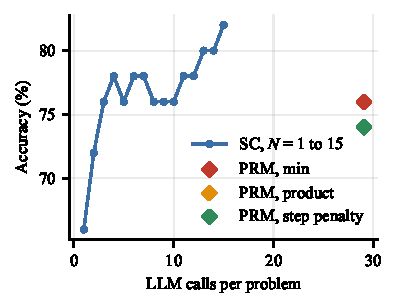
\includegraphics{figures/fig_calls.pdf}\caption{}\end{subfigure}\hfill
  \begin{subfigure}{0.49\linewidth}\centering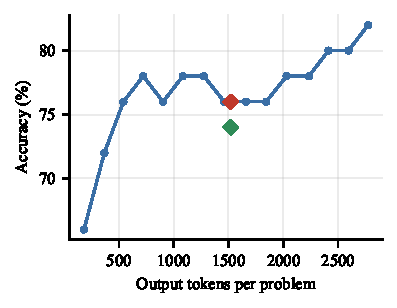
\includegraphics{figures/fig_tokens.pdf}\caption{}\end{subfigure}
  \caption{Accuracy against (a) LLM calls per problem and (b) output tokens per problem, generated plus judge, on the 50 problems. The self-consistency (SC) curve votes over the first $N$ of 15 sampled paths, and each diamond is one PRM-BoN-5 aggregation rule. The product and step-penalty diamonds coincide.}
  \label{fig:scaling}
\end{figure}

\begin{table}[t]
  \centering
  \small
  \caption{Paired comparison of each PRM rule against SC@5 and SC@15 on the same 50 problems. A PRM win is a problem the PRM rule answered correctly and the baseline did not. The difference is PRM accuracy minus baseline accuracy in percentage points (pp), with a paired bootstrap 95\% CI.}
  \label{tab:paired}
  \begin{tabular}{lrrrrrc}
    \toprule
    Comparison & \shortstack{PRM\\wins} & \shortstack{Baseline\\wins} & \shortstack{Both\\right} & \shortstack{Both\\wrong} & \shortstack{Difference\\(pp)} & \shortstack{95\%\\CI} \\
    \midrule
    min vs SC@5 & 0 & 0 & 38 & 12 & $0$ & [$0$, $0$] \\
min vs SC@15 & 0 & 3 & 38 & 9 & $-6$ & [$-14$, $0$] \\
product vs SC@5 & 1 & 2 & 36 & 11 & $-2$ & [$-10$, $+4$] \\
product vs SC@15 & 0 & 4 & 37 & 9 & $-8$ & [$-18$, $-2$] \\
step penalty vs SC@5 & 1 & 2 & 36 & 11 & $-2$ & [$-10$, $+4$] \\
step penalty vs SC@15 & 1 & 5 & 36 & 8 & $-8$ & [$-18$, $0$] \\
\bottomrule

  \end{tabular}
\end{table}

\paragraph{Only the gap to SC@15 exceeds sampling noise.} One problem is 2 percentage points (pp) of accuracy on 50 problems, so each method's 95\% CI spans 20 to 26 pp (Table~\ref{tab:results}) and the per-method intervals all overlap. The paired comparison removes the problem-to-problem variation that both methods share (Table~\ref{tab:paired}). Against SC@5 the PRM rules won at most 1 problem and lost at most 2, and every paired CI contains zero, because both methods choose among the same 5 paths and disagree on 3 problems at most. Against SC@15 the PRM rules won at most 1 problem and lost 3 to 5, and the paired CI for product, $[-18, -2]$ pp, excludes zero. We conclude that the PRM rules are indistinguishable from SC@5 on this sample and that SC@15 is better than product-pooled PRM search.

\section{Path Score Aggregation Ablation}
\label{sec:ablation}

\begin{table}[t]
  \centering
  \small
  \caption{Aggregation rules over the same judged 5-path pools. Tie rate is the share of problems where more than one path shared the best path score, so the final answer came from the vote among them. The last row multiplies the judge's probability of VALID at each step.}
  \label{tab:ablation}
  \begin{tabular}{lccc}
    \toprule
    Aggregation rule & Penalty weight $\lambda$ & Accuracy (\%) & Tie rate (\%) \\
    \midrule
    min & -- & 76 & 90 \\
product & -- & 74 & 52 \\
step penalty & 0.0 & 72 & 72 \\
step penalty & 0.5 & 74 & 72 \\
step penalty & 2.0 & 74 & 72 \\
product of $p_t$ (verdict logits) & -- & 72 & 0 \\
\bottomrule

  \end{tabular}
\end{table}

\paragraph{Min-pooling tied on most problems, so it reduced to majority voting.} With binary step scores $S_{\min}$ takes only the values $+1$ and $-1$, so all paths with no INVALID step tie at $+1$ and selection falls to the vote among them. Min tied on \tieMin\% of problems (Table~\ref{tab:ablation}). The filter changes the answer only when a pool mixes passing and failing paths and the passing paths vote differently from all 5. Of the \mixedPools{} mixed pools, this happened on \minChangedAnswer{} problems, and SC@5 was wrong on all 3 with PRM-min also wrong (Table~\ref{tab:paired}). On the \allValidPools{} pools where every path passed and the \allInvalidPools{} where every path failed, filter-then-vote is exactly SC@5. The vote among tied paths keeps min at SC@5 accuracy, since a tie-break by path order would select a single sampled path on \tieMin\% of problems.

\paragraph{Product and step penalty rank paths by length once INVALID counts are equal.} Writing $V$ and $I$ for a path's number of VALID and INVALID steps, the product rule gives $S_{\text{prod}}=0.99^{V}\,0.01^{I}$. Product behaves like min under binary scores, because for any path shorter than 458 steps a path with $I=0$ scores at least $0.99^{T}>0.01$ and a path with $I\ge 1$ at most $0.01$, so both rules separate the same passing and failing paths. Product then prefers the shorter of two paths with equal $I$, since each extra VALID step multiplies the score by 0.99, so a tie needs equal $I$ and equal length, which lowered the tie rate to \tieProduct\%. The step penalty mean $(V-I)/T$ is 1 for every path with $I=0$, so those paths tie, which gave \tiePenTwo\% ties. At $\lambda=0$ the mean alone ranks paths, and one INVALID step in a long path costs less than in a short one, so a long flawed path can outrank a short one with the same error. A positive $\lambda$ makes the count $I$ decide first, and $\lambda=0.5$ and $\lambda=2$ selected the same answers (\accPenTwo\% against \accPenZero\% at $\lambda=0$). Product and step penalty lost 2~pp to min, likely because a strict score order lets the judge's errors decide (Section~\ref{sec:failures}), whereas min leaves most decisions to the vote.

\paragraph{Judge probabilities removed ties and lost accuracy.} For the bonus rule we took the raw logits $z_{\text{V}}$ and $z_{\text{I}}$ of the tokens VALID and INVALID at the judge's first verdict token and set the step probability $p_t=e^{z_{\text{V}}}/(e^{z_{\text{V}}}+e^{z_{\text{I}}})$, then multiplied the $p_t$ along the path. We expected a continuous score to separate the paths that binary scores tie. It did, with a \tieLogprob\% tie rate, but accuracy fell to \accLogprob\% (Table~\ref{tab:ablation}). The thresholded $p_t$ agreed with the text verdict on \agreeLogprob\% of steps, so the probabilities add only the judge's confidence within a verdict, and selecting on that confidence replaces the vote with a ranking that no label was used to fit.

\section{Failure Mode and Judge Error Analysis}
\label{sec:failures}

\paragraph{Case 1, judge false positive. The judge passed a path with two flawed steps.} In problem \texttt{gsm8k\_test\_09}, candidate 3, John drives home for 4 hours after 3 hours out. The path computed the last leg as ``80 mph $\times$ 2 hours = 160 miles'' although only 1.5 hours remain, then added the outbound and return distances to get 355 miles where the answer is 45. The judge marked all 5 steps VALID, with rationales such as ``The arithmetic is correct and the distances add up as stated'', because each multiplication is correct and local validity checks the arithmetic of a step before its use of the question. This was the only path in the pool with no INVALID step, so all three PRM rules selected the wrong answer 355.

\paragraph{Case 2, judge false negative. The judge rejected a correct path for a redundant step.} In problem \texttt{gsm8k\_test\_02}, candidate 4, the path reached the correct 3 bolts and then multiplied by ``1 robe''. The judge marked that step INVALID with the rationale ``The problem asks for the total number of bolts for one robe, not for multiple robes'', which objects to the step's relevance although its arithmetic is correct. Under min this path scores $-1$ and leaves the vote, and it cost no accuracy because the other 4 paths also answered 3.

\paragraph{Case 3, shared flawed premise. Shared misreadings pass every step.} In problem \texttt{gsm8k\_test\_13}, Carlos earns \$7.50 a year from a \$90 tree and the question asks when he starts earning money. Candidates 0, 2 and 4 each computed 90 / 7.5 = 12 years, the break-even year, where the answer is 13. Every step of the three paths is arithmetically correct, so the judge passed all of them, the paths outvoted the rest, and every method including greedy decoding answered 12. A verifier that assumes the preceding steps are correct cannot see an error in reading the question that all paths share.

\begin{table}[t]
  \centering
  \small
  \caption{Hand audit of \auditN{} judged steps, 15 drawn from the judge-INVALID steps and 20 from the judge-VALID steps, labelled blind to the verdict. INVALID is the positive class, giving precision \auditPrecision\% and recall \auditRecall\% for INVALID detection within the sample.}
  \label{tab:audit}
  \begin{tabular}{lcc}
    \toprule
     & Human INVALID & Human VALID \\
    \midrule
    Judge INVALID & \auditTP{} (true positive) & \auditFP{} (false positive) \\
    Judge VALID & \auditFN{} (false negative) & \auditTN{} (true negative) \\
    \bottomrule
  \end{tabular}
\end{table}

\paragraph{The judge over-flagged steps and missed none in the audit.} The judge labelled \stepsInvalidPct\% of all \judgeCalls{} steps INVALID, so a random sample would hold few INVALID steps, and we drew 15 from the judge-INVALID steps and 20 from the judge-VALID steps. In Table~\ref{tab:audit} a flawed step marked VALID, as in the first case, counts as a false negative, since INVALID is the positive class. Precision for INVALID was \auditPrecision\% and recall \auditRecall\% within this sample. Because the strata were sampled at different rates, these are rates within the sample and not over all steps. Most false positives were correct steps the judge rejected for relevance, e.g.\ a step that restates a quantity or plans the next computation, as in the second case above. The false-negative cell is zero because the 20 judge-VALID draws contained no flawed step, which bounds the miss rate among VALID verdicts at 15\% (3/20, the rule of three). The first and third cases show that such misses exist outside the sample.

\paragraph{A stronger judge catches arithmetic errors, and self-verification would share the generator's misreadings.} The 7B judge caught arithmetic and unit errors that the 1.5B generator made, e.g.\ adding liters of drink to liters of water, which is consistent with its larger capacity. Its errors were of a different kind, i.e.\ rejecting correct steps for relevance and passing steps whose arithmetic is right but whose use of the question is wrong (first and third cases). If the 1.5B generator verified its own steps, we would expect its errors to follow the errors it makes when generating. It would then pass the shared misreadings that majority voting already selects, and lower arithmetic accuracy would pass more calculation errors, so the filter would remove few of the paths the vote would choose.

\section{Test-Time Compute Efficiency}
\label{sec:compute}

\paragraph{PRM-BoN-5 fits a budget of 10 greedy runs, and self-consistency with 11 paths does better within it.} Greedy decoding produced \greedyTokens{} output tokens over the 50 problems, so the budget of 10 times greedy is \budgetTenX{} tokens. PRM-BoN-5 spent \prmGenTokens{} generated plus \prmJudgeOut{} judge output tokens, i.e.\ \prmSpent{} tokens, within the budget. Sampled paths averaged \genPerSample{} tokens, so self-consistency fits up to $N=\largestSCN$ paths (\largestSCN{} $\times$ 50 $\times$ \genPerSample{} $\le$ \budgetTenX), which reached \accSCeleven\% against \accPRMmin\% for PRM-min (Figure~\ref{fig:scaling}b). SC@15 used \scTokensFifteen{} tokens and exceeds the budget.

\paragraph{Output tokens understate the judge's cost.} Each of the \judgeCalls{} judge calls read the question and all preceding steps, a mean of \judgeInPerCall{} prompt tokens against \judgeOutPerCall{} output tokens, a ratio of \judgeInOverOut. The judge also has 7B parameters against 1.5B for the generator, so each of its tokens costs more. Judging took \judgeTimeOverSC{} times the sampling time of SC@5 (Table~\ref{tab:results}, PRM time minus SC@5 time over SC@5 time). Calls show the same asymmetry, with \callsPRMperProblem{} calls per problem for PRM-BoN-5 against 15 for SC@15 (Figure~\ref{fig:scaling}a).

\paragraph{We recommend spending the budget on sampling.} At every compute level we measured, the self-consistency curve lay at or above the PRM points (Figure~\ref{fig:scaling}). Extra paths raise the chance that the correct answer is present and that it holds the majority. This judge's verdicts re-rank a fixed pool and err in both directions (Section~\ref{sec:failures}). \citet{snell2024scalingllmtesttimecompute} found that verifier-guided search improves accuracy when the verifier is accurate, which our audit shows this prompted judge is not.

\section{Reproducibility and Limitations}
\label{sec:repro}

\paragraph{Reproducibility.} The run used one NVIDIA L4 GPU on Google Colab with both models on the same GPU. The two models occupied 8.7 GiB of the 22.5 GiB of GPU memory during the run, and the run took 55 minutes of wall-clock time from launch to exit, including model loading. The seed protocol is in Section~\ref{sec:results}. We used PyTorch 2.14.1, Transformers 5.22.1 and bitsandbytes 0.50.2.

\paragraph{A prompted verifier has no trained notion of step correctness.} A PRM trained on human step labels such as PRM800K \citep{lightman2023letsverifystepstep} learns to predict whether a step is correct from many labelled examples of the same task, and its score estimates the probability that the solution is still on track. A prompted judge has only an instruction, so its verdict reflects what the instruction emphasises, here arithmetic, and its notion of an error is not fitted to human labels, which our audit shows as rejections for relevance. Its VALID probabilities are not fitted to step labels, and under local validity it evaluates each step without the question's global constraints, both of which a trained PRM learns from labelled data. Our evidence comes from one seed per problem, 50 problems, one judge prompt and one sampling temperature, and none of these was varied.

\bibliographystyle{plainnat}
\bibliography{ref}

\end{document}
